\documentclass[12pt,a4paper]{article}
\usepackage[margin=0.5in]{geometry} % custom margins
\usepackage{graphicx}
\graphicspath{ {./Images/} }
\usepackage{array,mathtools}
\usepackage{listings}

% When writing indented paragraphs:
% \usepackage{indentfirst}

% To supress page numbers:
% \usepackage{nopageno}

\begin{document}
\begin{center}
    
\includegraphics[width=\textwidth]{./Images/Header.jpeg}
    \vfill
    \textbf{\Large{Report for Experiment \#1\\
    Eight Bit Adder}}
    \vfill
    Trevor Smith\\
    February 10, 2022
    \vfill
\end{center}

\newpage

\section*{Prelab:}

\begin{enumerate}
	\item
$\begin{array}[t]{r|r|r|r}
	a & b & f & ovf \\ \hline
	8'd0    & 8'd0    & 0000\ 0000 & 0 \\
	8'd12   & 8'd34   & 0000\ 1110 & 0 \\
	-8'd12  & -8'd34  & 1101\ 0010 & 0 \\
	8'd100  & -8'd50  & 0011\ 0010 & 0 \\
	-8'd100 & 8'd50   & 1100\ 1110 & 0 \\
	8'd100  & 8'd100  & 1100\ 1000 & 1 \\
	-8'd100 & -8'd100 & 1\ 0011\ 1000 & 1 \\
	8'd3    & 8'd0    & 0000\ 0011 & 0 \\
 \end{array}$ \\ \\
 For -100 -100 I'm aware the 9th bit would be chopped off, just showing
 the theoretical value.
 
 	\item
$\begin{array}[t]{r|c|c|}
	ab \setminus^f & 0 & 1 \\ \hline
	00 & 0 & 1 \\
	01 & 0 & 0 \\
	11 & 1 & 0 \\
	10 & 0 & 0 \\
\end{array}$ \\
Where A=a[0], B=b[0], f=f[0], \\
$$ \overline{AB}f + AB\overline{f} = ovf $$

	\item
		We almost test every bit, which is somehow easier with two's complement
		since the minus sign has a tendency to make zeros into ones. However,
		we never test the 1's bit. As such, I added 3 + 0 as a test in the above
		table.
\end{enumerate}

\section*{Results and Analysis:}

An eight-bit adder was fully implemented, tested, and verified using the Vivado IDE.
After some fiddling, the outputs were all found to match expected values.
The program was then ported to the PYNQ board, using provided mappings, and tested
in real-time. While the base implementation of the addition was just a wrapper for
verilog's '+' operator, the overflow was developed and tested as well, which transformed
the base verilog adder into a two's complement eight-bit adder. \\


\section*{Conclusion and Recommendations:}

An eight-bit adder was successfully implemented and tested. 
The most significant challenge in completing this lab was by far the Vivado software 
and infamiliar verilog syntax. As such, this was a useful learning opportunity.
In the future, more advanced functions and programs will be possible based on
growing fluency with these tools. 

\newpage
\section*{Appendices:}

\subsection{Appendix A: Design Program Files}

\begin{lstlisting}

module eightbit_adder(
    input [7:0]a,
    input [7:0]b,
    output [7:0]f,
    output ovf
    );

    assign f = a + b;
    assign ovf=f[7]? ~(a[7]|b[7]):a[7]&b[7];
    
endmodule


module adder8_tb();

    //Inputs
    reg [7:0]a;
    reg [7:0]b;
    //Outputs
    wire [7:0]f;
    wire ovf;
    
    //UUT
    eightbit_adder UUT
       (.a(a),
        .b(b),
        .f(f),
        .ovf(ovf)
    );
    
    initial
        begin
            
            #200;
            a=8'b1;
            b=8'b1;
            
            #100;
            a = 8'd12;
            b = 8'd34;

            #100;
            a = -8'd12;
            b = -8'd34;

            #100;
            a = 8'd100;
            b = -8'd50;

            #100;
            a = -8'd100;
            b = 8'd50;

            #100;
            a = -8'd12;
            b = -8'd34;

            #100;
            a = 8'd100;
            b = 8'd100;

            #100;
            a = -8'd100;
            b = -8'd100;

        end
        
endmodule
\end{lstlisting}

\newpage
\subsection{Appendix B: Output Screen Capture}

\begin{figure}[h]
	\centering
	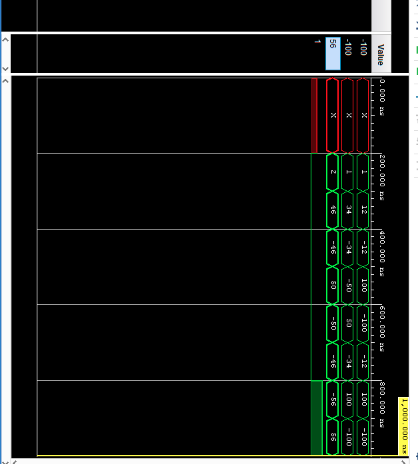
\includegraphics{image}
	\caption{Test bench output}
\end{figure}

\end{document}
